\documentclass[a4paper,12pt,oneside,openany,table,xcdraw]{article}

\usepackage{setspace}
\usepackage{multirow}
\usepackage{hyperref}
\usepackage{caption}
\usepackage{indentfirst}

\usepackage[brazilian]{babel}
\usepackage[utf8x]{inputenc}
\usepackage{amsmath, graphicx, mathptmx, enumerate}
\usepackage{float, verbatim}
\usepackage[colorinlistoftodos]{todonotes}
\usepackage{makeidx} % Para o sumário
\usepackage{geometry}

\geometry{a4paper, hmargin={3cm, 3cm}, vmargin={3cm, 2cm} }
\setlength{\parindent}{1.0cm}

\begin{document}
\newcommand{\thedepartment}{Faculdade de Engenharia Elétrica}
\newcommand{\thecourse}{FEELT}
\newcommand{\thetitle}{TENSÕES, CORRENTE E POTÊNCIAS EM CIRCUITO SÉRIE, FATOR DE POTÊNCIA E CORRENTE ALTERNADA SENOIDAL - USO DE MEDIDORES ANALÓGICOS E DIGITAIS}
\newcommand{\thetype}{Relatório da Disciplina de Circuitos Elétricos II}
\newcommand{\theproftitle}{Bacharel em Engenharia Elétrica}
\newcommand{\thestudent}{Lesly Viviane Montúfar Berrios\\
\centering11811ETE001}
\newcommand{\theadvisor}{Prof. Wellington Maycon Santos Bernardes}
\newcommand{\thecity}{Uberlândia}

\thispagestyle{empty}\newcommand*{\themonth}{\ifthenelse{\the\month < 2}{Janeiro }
                  {\ifthenelse{\the\month < 3}{Fevereiro }
                  {\ifthenelse{\the\month < 4}{Março }
                  {\ifthenelse{\the\month < 5}{Abril }
                  {\ifthenelse{\the\month < 6}{Maio }
                  {\ifthenelse{\the\month < 7}{Junho }
                  {\ifthenelse{\the\month < 8}{Julho }
                  {\ifthenelse{\the\month < 9}{Agosto }
                  {\ifthenelse{\the\month < 10}{Setembro }
                  {\ifthenelse{\the\month < 11}{Outubro }
                  {\ifthenelse{\the\month < 12}{Novembro }{Dezembro }}}}}}}}}}}}
                  
\begin{titlepage}
\begin{center}

	\vspace{-0.5cm}

  \begin{figure}[hbt!]
		\begin{center}
		   
\includegraphics[width=2.8cm]{ufu-logo.png}
		\end{center}
	\end{figure}
 	%\vspace{-4cm}

%\begin{doublespacing}

  \Large{\textbf{Universidade Federal de Uberlândia}}\\
  \large{\thedepartment}\\
  \large{\thecourse}\\


\vspace{5.8cm}
  \par
  \large\textbf{\thetitle}
\vspace{5.8cm} 

%\end{doublespacing}
  \par
  \thetype\\
  por\\
  %\hspace{2cm}\large{}\\

\vspace{0.8cm}
\par
  \normalsize{\thestudent}\\ [2cm]
  \theadvisor

\par\vfill
  \thecity, \themonth / \the\year

\end{center}

\end{titlepage}

%% Comeca o documento !

\onehalfspacing
\tableofcontents % sumário
\newpage

\section{Objetivos} % 2,5%
Montar um circuito série \emph{RLC}, energizá-lo com tensão alternada senoidal, realizar medições usando
equipamentos analógicos e digitais, efetuar desenvolvimentos teóricos e cálculos numéricos confrontando os
resultados teóricos com aqueles obtidos experimentalmente.

\section{Introdução teórica} % 5%

\subsection{Análise do circuito}
O circuito a ser analisado neste experimento é descrito na Figura \ref{circuito} e do conhecimento teórico de circuitos em série tem-se os cálculos descritos pelas Equações (\ref{Z}) e (\ref{I}).

\begin{figure}[H]
\centering
\captionsetup{font=scriptsize}
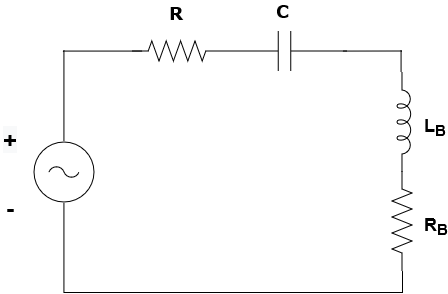
\includegraphics[width=11cm]{circuito}
\caption{Montagem experimental.}
\label{circuito}
\end{figure}

A impedância total na forma fasorial é descrita como na Equação \ref{Z}, assim tomando-se o módulo é possível descrever a corrente como na Equação \ref{I}.
\begin{equation}\label{Z}
\dot{Z}=(R+R_{B}) + j\, (X_{L_{B}}+ X_{C})
\end{equation}
\begin{gather*}
Z = \sqrt{(R+R_{B})^2 + (X_{L_{B}}+ X_{C})^2 } \\
V = Z\, I
\end{gather*}
\begin{equation}\label{I}
I = \dfrac{V}{\sqrt{(R+R_{B})^2 + (X_{L_{B}}+ X_{C})^2 }}
\end{equation}

\subsection{Potências Eficazes}
As potências ativa, reativa e aparente eficazes podem ser calculadas, respectivamente, pelas Equações (3), (4) e (5). 
\begin{gather}
P=V_{ef}\cdot I_{ef}\cdot cos\theta\\
Q=V_{ef}\cdot I_{ef}\cdot sen\theta\\
S=V_{ef}\cdot I_{ef}
\end{gather}

\section{Preparação}
\subsection{Materiais e ferramentas} % 2,5%
\begin{enumerate}[1 - ]
\item \emph{Fonte}\\
Alimentará todo o circuito.

\item \emph{Variador de tensão (Varivolt)}\\
O equipamento permitirá obter o valor desejado de corrente a partir da regulagem correta da tensão fornecida pela fonte. Também chamado de autotransformador.

\item \emph{Medidor eletrônico KRON Mult K}\\
Possibilita encontrar a medição da potência
real (P) - vatímetro, reativa (Q) e aparente (S) do circuito. Ele também possui função de cofasímetro, instrumento elétrico que mede o fator de potência (fp, $cos\theta$) ou o ângulo da impedância $\theta$ do circuito, para um circuito com a impedância $Z = Z\angle \theta$.

\item \emph{Conectores}\\
Foram utilizadas pontas de provas para a verificação das grandezas nos multímetros e pontas de prova específicas para multímetro. Para as conexões no circuito foi utilizado majoritariamente cabos banana-banana.

\item \emph{Multímetro}\\
Utilizado para medir a resistência R, capacitância C e gradezas do conjunto L e $R_L$ especificados no experimento.

\item \emph{Amperímetro analógico AC}\\
Instrumento de maior precisão.

\item \emph{Voltímetro analógico AC}\\
Instrumento de maior precisão.

\item \emph{Osciloscópio}\\
Utilizado obter informações da forma de onda ($V_{pp}$,$V_{max}$, $V_{rms}$).

\item \emph{Reostato R}\\
Reostato com potência nominal de aproximadamente 1kW.

\item \emph{Capacitor C}\\
Reostato com potência nominal de aproximadamente 1kW.

\item \emph{Bobina B}\\
O valor medido da indutância da bobina B (reator para lâmpada vapor de sódio) realizada
recentemente (Agosto/2019) é de 160 mH e resistência interna de 3,8 ohms.

\end{enumerate}

\subsection{Montagem} % 2,5%

%\begin{enumerate}[1)]
%\item \emph{Montando o circuito}\\
Realize a montagem informada na Figura \ref{fig1}, com os parâmetros R, C, L, RL, V e f (preenchendo as
Tabelas 1 e 2). 

\begin{figure}[H]
\centering
\captionsetup{font=scriptsize}
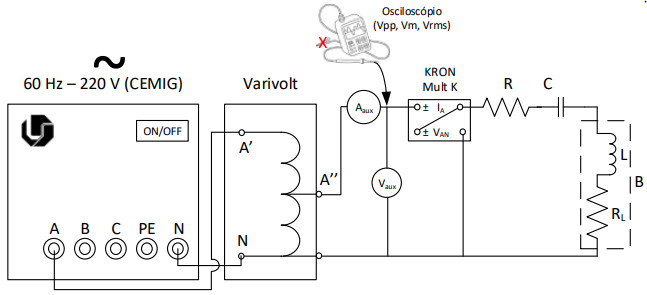
\includegraphics[width=14.5cm]{fig1}
\caption{Montagem experimental.}
\label{fig1}
\end{figure}

%\end{enumerate}

\section{Análise sobre segurança} % 2,5%
Os óculos de segurança são Equipamentos de Proteção Individual (EPIs) e são utilizados para a proteção da área ao redor dos olhos contra qualquer tipo de detrito estranho, que possa causar irritação ou ferimentos. Também protegem contra faíscas, respingos de produtos químicos, detritos, poeira, radiação e etc \cite{safe}.
É importante a utilização desse equipamento durante os experimentos a fim de evitar qualquer dano, além de preparar o profissional para o manejo correto e seguro de qualquer equipamento.
Além disso, foi de extrema importância a presença do professor ou técnico na verificação da montagem do circuito antes de energizá-lo. Assim, reduziu-se riscos de curtos-circuitos ou sobrecarga na rede.

\section{Cálculos, análise dos resultados e questões} % (quando houver) (70%)

\begin{enumerate}[1 - ]
\item Complete a Tabela \ref{tab1} com os dados do Caso A, sendo $V_{ef}=100V$ e $R=100\Omega$ (teórico).

\begin{table}[h]
\centering
\def\arraystretch{1.35}
\captionsetup{font=scriptsize}
\captionof{table}{Parâmetros reais da montagem do primeiro caso.} \label{tab1}
\begin{tabular}{|c|c|c|c|c|c|}
\hline
$R [\Omega]$ & $C [\mu F]$ & $L [mH]$ & $R_L [\Omega]$ & $V [volts]$ & $f [Hz]$ \\ \hline
       100      &    45,9     &    160      &         3,8       &      99,4       &     59,95     \\ \hline
\end{tabular}
\end{table}

\item Complete a Tabela \ref{tab2} com os dados do Caso B, sendo $V_{ef}=50V$ e $R=20\Omega$ (teórico). \\

\begin{table}[h]
\centering
\def\arraystretch{1.35}
\captionsetup{font=scriptsize}
\captionof{table}{Parâmetros reais da montagem do segundo caso.} \label{tab2}
\begin{tabular}{|c|c|c|c|c|c|}
\hline
$R [\Omega]$ & $C [\mu F]$ & $L [mH]$ & $R_L [\Omega]$ & $V [volts]$ & $f [Hz]$ \\ \hline
       20      &    45,9     &    160      &         3,8       &       49,39      &     60,00     \\ \hline
\end{tabular}
\end{table}

\item Ajuste a tensão de saída do autotransformador (varivolt) de maneira a obter a tensão solicitada para o voltímetro e anote os valores medidos na Tabela \ref{tab3} (para ambos os casos, A e B). Os resultados são obtidos por meio dos cálculos apresentados na introdução teórica. \\
\begin{table}[H]
\centering
\def\arraystretch{1.35}
\captionsetup{font=scriptsize}
\captionof{table}{Erro percentual das duas montagens.} \label{tab3}

\resizebox{\textwidth}{!}{ %
\begin{tabular}{|c|c|c|c|c|c|c|c|c|c|c|c|c|}
\hline
\multirow{3}{*}{Valores} & \multicolumn{9}{c|}{Medições}                                                                         & \multicolumn{3}{c|}{Cálculos}          \\ \cline{2-13} 
                         & $V_{ef}$ & I       & $cos\theta$ & $V_R$   & $V_C$   & $V_{(L+R_L)}$ & P       & S        & Q         & $\theta^{[1]}$ & $S^{[2]}$ & $Q^{[3]}$ \\ \cline{2-13} 
                         & {[}V{]}  & {[}A{]} & {[}fp{]}    & {[}V{]} & {[}V{]} & {[}V{]}       & {[}W{]} & {[}VA{]} & {[}VAr{]} & $[^{\circ}]$   & {[}VA{]}  & {[}Var{]} \\ \hline
\multicolumn{13}{|c|}{Caso A}                                                                                                                                             \\ \hline
Medidos                  & 99,40    & 0,932   & 0,988       & 93,10   & 54,36   & 69,40         & 90,90   & 92,01    & 14,23  &   8,89           & 92,64     & 14,25     \\ \hline
Calculados               & 100      & 0,963   & 0,999       &   96,30      &  55,65    & 58,19  & 96,20    & 96,30    & 4,30   &   2,56           &  96,30    &  4,30         \\ \hline
Erros (\%)               & -0,60       & -3,34   & -1,113   &  -3,44  &  -2,37   &  16,15        & -5,83     & -3,95    & 69,77 &   71,20          & -3,95     &  69,82         \\ \hline
\multicolumn{13}{|c|}{Caso B}                                                                                                                                             \\ \hline
Medidos                  & 49,39    & 1,702   & 0,873      & 34,16   & 99,8    & 124,00        & 73,10   & 84,00    & 41,39     & 29,19          & 84,06     & 41,38     \\ \hline
Calculados               & 50,00   & 2,089    & 0,994     & 41,78   &120,72 & 126,24        & 103,82  & 104,45   &  11,41         &      6,27      &    104,45     &  11,45        \\ \hline
Erros (\%)               &-1,24     &-22,74   &-13,91     & -22,30  & -20,97 & -1,81          & -42,02  & -24,34    &  72,43         &   78,48       &    -24,26       &  72,32       \\ \hline
\end{tabular} % 
}
\end{table}

\noindent\text{[1]} Calcule o valor medido de $\theta$ à partir do fator de potência, ou seja, $\theta = arccos(fp)$. \\
\noindent\text{[2]} Calcule a potência aparente S à partir dos valores medidos para V e I, ou seja, $S=V\times I$. \\
\noindent\text{[3]} Calcule a potência reativa Q à partir do triângulo de potência, ou seja, $Q^2=S^2-P^2$. 

Calculando-se as impedâncias sobre o capacitor e indutor tem-se, respectivamente, $X_{C}=57,79\Omega$ e $X_{L_B}=60,31\Omega$.  Ademais, para a bobina $Z_B=\sqrt{R_B^2+L_B^2}=60,43\Omega$. O cálculo do fp foi relizado pela relação do triângulo de impedâncias.

Para o caso A, do cálculo do módulo da impedância por meio da Equação (\ref{Z}) tem-se $Z=103,8284\Omega$, logo $I=0,963A$.
Já para o caso B, do cálculo do módulo da impedância por meio da Equação (\ref{Z}) tem-se $Z=23,9339\Omega$, logo $I=2,089A$.

\item Ligue o osciloscópio (canal CH1), automatize o trigger e colete $V_{pp}$, $V_m$ e $V_{rms}$. Registre a imagem.
Use a função MEASURE $>$ TODAS MED para o equipamento realizar os cálculos práticos.

\begin{figure}[H]
\centering
\captionsetup{font=scriptsize}
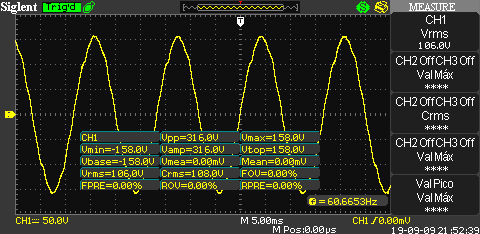
\includegraphics[width=11cm]{osc1}
\caption{Imagem do osciloscópio para o Caso A.}
\label{osc1}
\end{figure}
\begin{figure}[H]
\centering
\captionsetup{font=scriptsize}
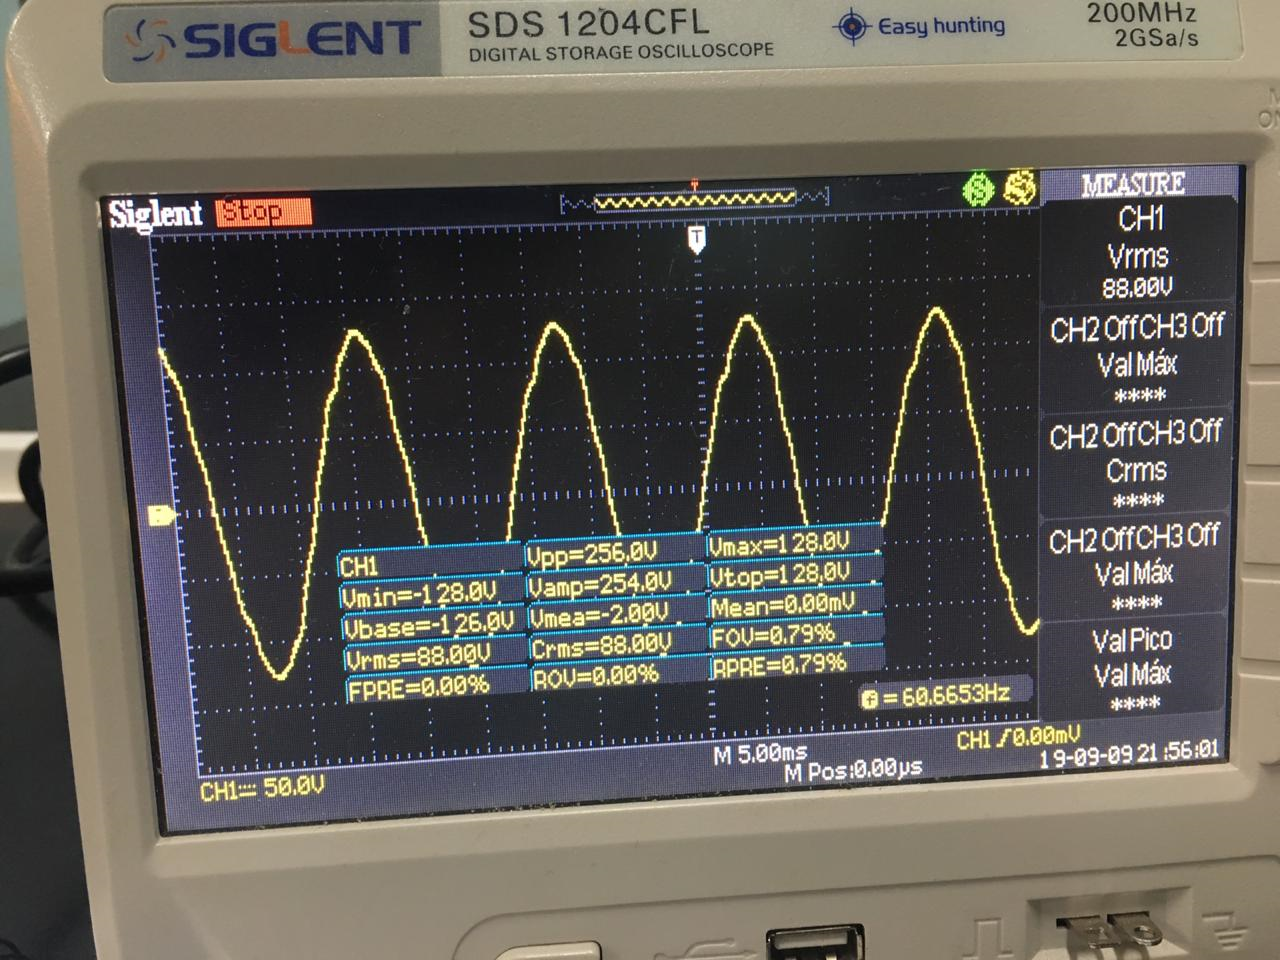
\includegraphics[width=11cm]{osc2}
\caption{Imagem do osciloscópio para o Caso B.}
\label{osc2}
\end{figure}

\item Comparação dos equipamentos de medição analógicos e digitais \\
\begin{table}[H]
\centering
\def\arraystretch{1.35}
\captionsetup{font=scriptsize}
\captionof{table}{Comparativo das medições para o Caso A.} \label{cA}
\begin{tabular}{c|c|c|}
\cline{2-3}
                                              & \textit{V {[}V{]}} & \textit{I {[}A{]}} \\ \hline
\multicolumn{1}{|c|}{KRON Mult K}             & 99,40              & 0,932              \\ \hline
\multicolumn{1}{|c|}{Analógico}               & 102,00             & 0,930              \\ \hline
\multicolumn{1}{|c|}{Osciloscópio}            & 106,00             & (1,06)             \\ \hline
\multicolumn{1}{|c|}{Erros Analógico (\%)}    & -2,62              & 0,21               \\ \hline
\multicolumn{1}{|c|}{Erros Osciloscópio (\%)} & -6,64              & -13,73             \\ \hline
\end{tabular}
\end{table}

\begin{table}[H]
\centering
\def\arraystretch{1.35}
\captionsetup{font=scriptsize}
\captionof{table}{Comparativo das medições para o Caso B.} \label{cB}
\begin{tabular}{c|c|c|}
\cline{2-3}
                                              & \textit{V {[}V{]}} & \textit{I {[}A{]}} \\ \hline
\multicolumn{1}{|c|}{KRON Mult K}             & 49,39              & 1,732              \\ \hline
\multicolumn{1}{|c|}{Analógico}               & 50,08              & 1,65               \\ \hline
\multicolumn{1}{|c|}{Osciloscópio}            &                    &                    \\ \hline
\multicolumn{1}{|c|}{Erros Analógico (\%)}    & 1,39               & 4,73               \\ \hline
\multicolumn{1}{|c|}{Erros Osciloscópio (\%)} &                    &                    \\ \hline
\end{tabular}
\end{table}

\item Manejo do equipamento \emph{KRON Mult K}\\
A regulagem do equipamento utilizando-se os parâmetros TP (Transformador de Potencial), TC (Transformador de Corrente) e TL (Transformador de Ligação) foi essencial, uma vez que é preciso informar ao equipamento que se trata de um circuito monofásico (1 fase + neutro), para isso configura-se $TL=0002$. TP e TC foram regulados a partir dos equipamentos analógicos pela relação descrita pela Equação \ref{TP} e \ref{TC}e conseguiu-se $TP=1,00$ e $TC=1,01$, para os quais os valores no equipamento digital também correspondem ao do analógico.
\begin{equation}\label{TP}
\dfrac{{TP}_{antigo}}{{TP}_{novo}}=\dfrac{V_{KRON}}{V_{analogico}}
\end{equation}
\begin{equation}\label{TC}
\dfrac{{TC}_{antigo}}{{TC}_{novo}}=\dfrac{I_{KRON}}{I_{analogico}}
\end{equation}

\end{enumerate}


\section{Simulação computacional} % (10%);

\subsection{Caso A}
Da simulação computacional tem-se as Figuras \ref{corrente1}, \ref{tensao-R1}, \ref{tensao-C1} e \ref{tensao-B1}.
\begin{figure}[H]
\centering
\captionsetup{font=scriptsize}
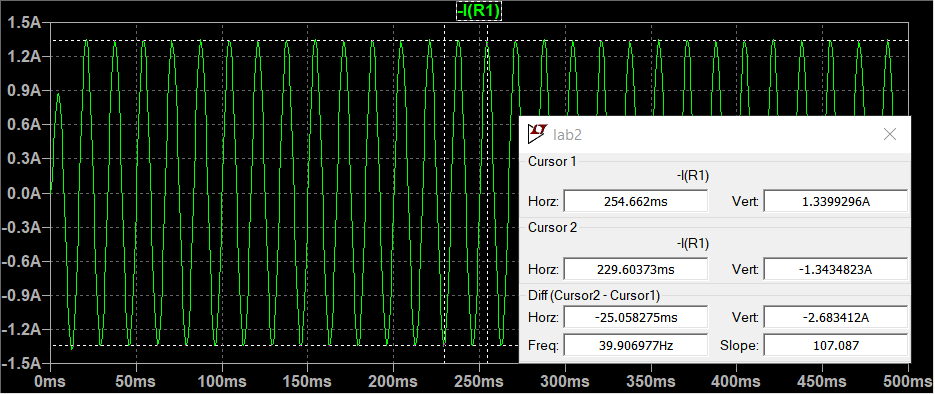
\includegraphics[width=11cm]{corrente1}
\caption{Corrente do circuito.}
\label{corrente1}
\end{figure}
\begin{figure}[H]
\centering
\captionsetup{font=scriptsize}
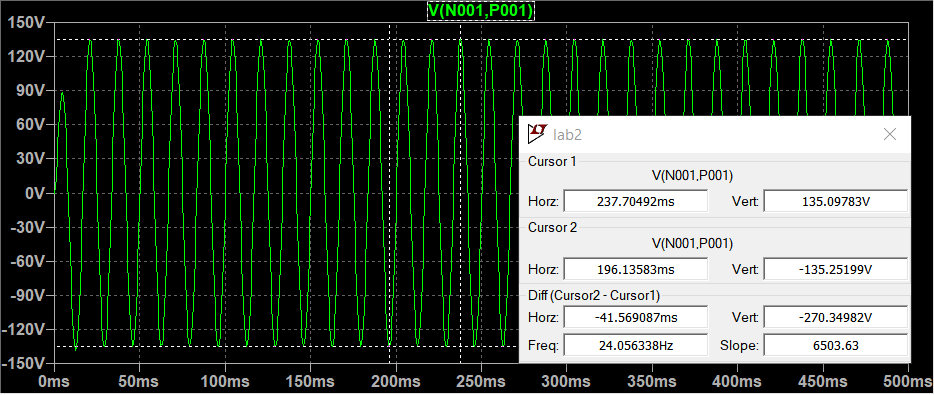
\includegraphics[width=11cm]{tensao-R1}
\caption{Tensão no resistor R.}
\label{tensao-R1}
\end{figure}
\begin{figure}[H]
\centering
\captionsetup{font=scriptsize}
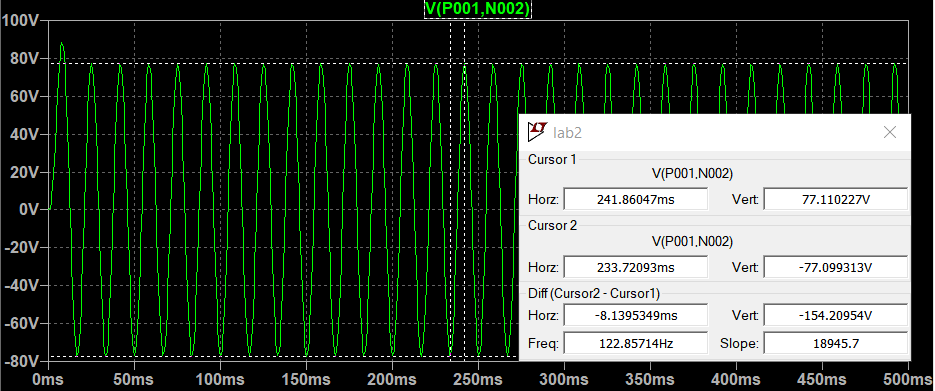
\includegraphics[width=11cm]{tensao-C1}
\caption{Tensão no capacitor C.}
\label{tensao-C1}
\end{figure}
\begin{figure}[H]
\centering
\captionsetup{font=scriptsize}
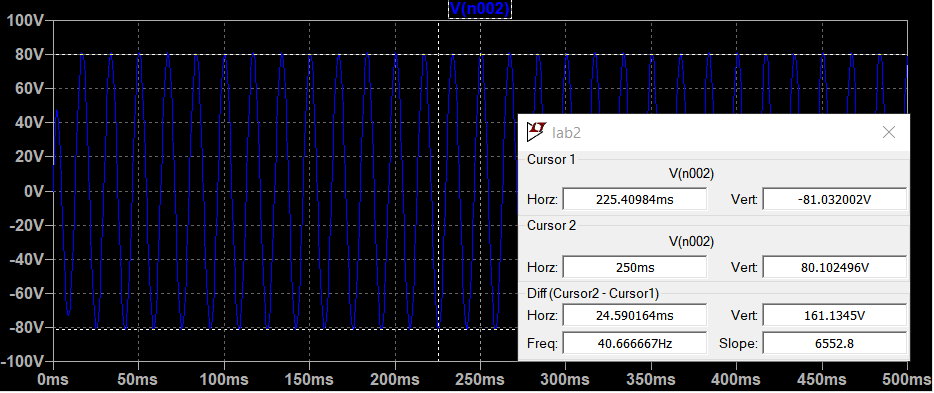
\includegraphics[width=11cm]{tensao-B1}
\caption{Tensão na bobina B.}
\label{tensao-B1}
\end{figure}

\subsection{Caso B}
Da simulação computacional tem-se as Figuras \ref{corrente2}, \ref{tensao-R2}, \ref{tensao-C2} e \ref{tensao-B2}.
\begin{figure}[H]
\centering
\captionsetup{font=scriptsize}
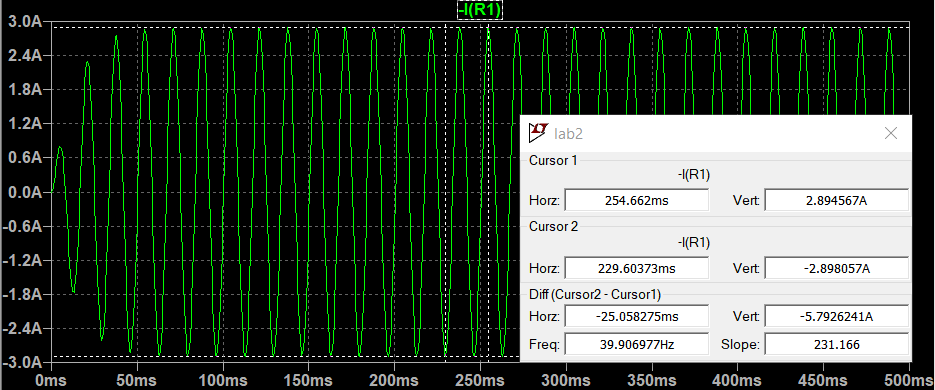
\includegraphics[width=11cm]{corrente2}
\caption{Corrente do circuito.}
\label{corrente2}
\end{figure}
\begin{figure}[H]
\centering
\captionsetup{font=scriptsize}
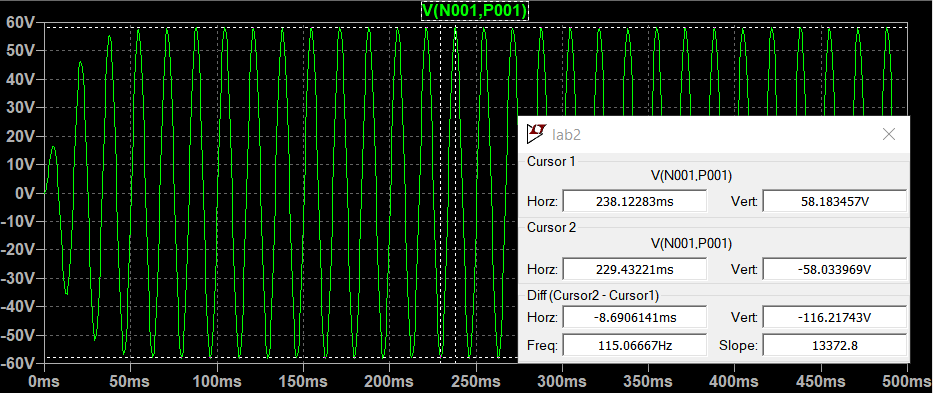
\includegraphics[width=11cm]{tensao-R2}
\caption{Tensão no resistor R.}
\label{tensao-R2}
\end{figure}
\begin{figure}[H]
\centering
\captionsetup{font=scriptsize}
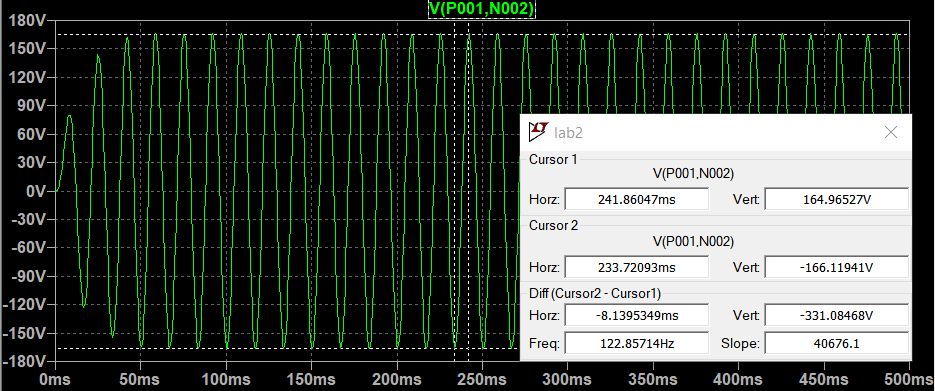
\includegraphics[width=11cm]{tensao-C2}
\caption{Tensão no capacitor C.}
\label{tensao-C2}
\end{figure}
\begin{figure}[H]
\centering
\captionsetup{font=scriptsize}
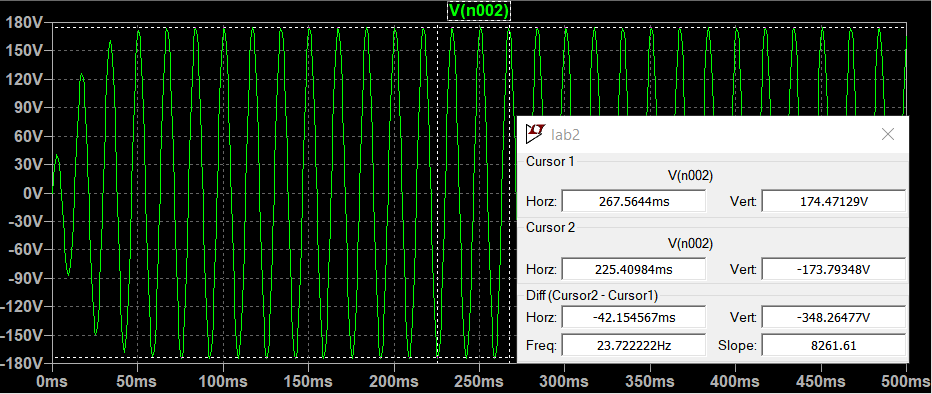
\includegraphics[width=11cm]{tensao-B2}
\caption{Tensão na bobina B.}
\label{tensao-B2}
\end{figure}

\section{Conclusões} % (no mínimo 10 linhas) (5%);
Este experimento trata-se da análise de um circuito série \emph{RLC} energizado com tensão senoidal, descrito pela Figura \ref{fig1}, . Calculou-se as impedâncias, corrente, tensão sobre cada componente a partir da análise das malhas, além das potências eficazes, por meio da análise teórica. Assim, foi possível a comparação com os valores obtidos experimentalmente tanto com medidores analógicos quanto com os digitais, o que é descrito pelas Tabelas \ref{cA} e \ref{cB}. Também foi importante a configuração do equipamento \emph{KRON Mult K} por meio dos parâmetros TL, TP e TC. 

Finalmente, a simulação computacional permitiu obter as medições com os dados experimentais dos componentes, dessa forma, identificou-se os erros associados aos equipamentos de medidas, seja por desregulagem ou erro do olho humano. Agrega-se a importância dos Equipamentos de Segurança Individual (EPI), uma vez que a utilização dos óculos durante o manejo dos componentes, mesmo que aparentemente ainda não sejam potenciais situações de risco, permite a criação do hábito de proteção e prevenção, uma característica essencial para o engenheiro na área de trabalho.


\newpage
\begin{thebibliography}{9} 
% Introdução
\bibitem{irwin}
    J. D. Irwin,
    “Análise de Circuitos Em Engenharia”, Pearson, $4^a$ Ed., 2000.

\bibitem{boylestad}
    R. L. Boylestad,
    “Introdução À Análise de Circuitos”, Pearson, $10^a$ Ed., 2004.

\bibitem{safe}
    SafetyTrabi,
    “Óculos de segurança: Saiba quando utilizar este EPI”, SafetyTrab, 2019.
 Disponível em:
 \url{https://www.safetytrab.com.br/blog/oculos-de-seguranca/}. Acesso em: ago. 2019.


\end{thebibliography}
\end{document}
